\documentclass[runningheads]{llncs}

\usepackage[T1]{fontenc}
\usepackage{amsmath}
\usepackage{graphicx}
\usepackage{booktabs}
\usepackage{xcolor}
\usepackage[nospace]{cite}
\usepackage{hyperref}
\usepackage{xurl}
\renewcommand\UrlFont{\color{blue}\rmfamily}
\urlstyle{rm}

\newif\ifanonymous
\anonymoustrue

\begin{document}

\title{News Publisher Reliability from Article Collections: A Publisher-Disjoint Evaluation}
\titlerunning{News Publisher Reliability from Article Collections}

\ifanonymous
  \author{Anonymous Author(s)}
  \authorrunning{Anonymous Author(s)}
  \institute{Affiliation withheld for double-blind review}
\else
  \author{%
  John Bianchi\inst{1}\orcidID{0009-0006-2582-1480} \and
  Manuel Pratelli\inst{2}\orcidID{0000-0002-9978-791X} \and
  Fabio Pinelli\inst{1}\orcidID{0000-0003-1058-6917} \and
  Marinella Petrocchi\inst{2,1}\orcidID{0000-0003-0591-877X}}
  \authorrunning{J. Bianchi et al.}

  \institute{%
  IMT School for Advanced Studies Lucca, 55100 Lucca, Italy\\
  \email{\{john.bianchi,fabio.pinelli\}@imtlucca.it}
  \and
  Institute of Informatics and Telematics, National Research Council (IIT-CNR),
  56124 Pisa, Italy\\
  \email{\{manuel.pratelli,marinella.petrocchi\}@iit.cnr.it}}
\fi

\maketitle

\begin{abstract}
Reliability ratings are assigned to news publishers, yet computational approaches often formulate the task as article-level classification, inheriting publisher labels at the article level and, in some cases, allowing the same publishers to appear in both training and test data. This mismatch creates a risk of publisher leakage and leaves unclear whether the reported performance generalizes to previously unseen outlets. We reformulate the task as publisher-level reliability inference from multiple articles. Our two-stage framework first derives a reliability prediction from each article and then aggregates these predictions to assign the publisher one of five ordinal reliability levels. We evaluate four transformer-based models using five-fold publisher-disjoint cross-validation on 19,476 English-language political news articles from 439 publishers annotated with NewsGuard scores. The best models achieve approximately 0.60 exact accuracy at the article level and 0.69 after aggregation at the publisher level. When predictions adjacent to the reference level are accepted, accuracy reaches 0.84 and 0.88, respectively, indicating that most errors remain local on the ordinal scale. Larger decoder-based models provide no consistent advantage over encoder-based models in this setting. We additionally examine how errors vary across publishers' political leanings, highlighting the importance of complementing aggregate performance with group-level error analysis. These results show that aggregating evidence across articles supports reliability estimation for unseen publishers while providing a stricter protocol for evaluating cross-publisher generalization.

\keywords{News source reliability \and
Transformer-based classification \and Cross-publisher generalization \and Political bias analysis}
\end{abstract}

\section{Introduction}
Assessing the reliability of news publishers has become increasingly important for limiting the spread of misleading or low-quality information. Professional organizations such as NewsGuard, the Global Disinformation Index, and Media Bias Fact Check evaluate news outlets according to journalistic standards including transparency, editorial accountability, factual accuracy, and correction practices, and despite methodological differences they exhibit substantial convergence~\cite{lin2023high,DBLP:conf/icwsm/PratelliP22}. These assessments are performed at the level of the publisher rather than of individual articles. Trained analysts produce them by hand, so the news outlets they never reach stay unrated.

A large body of computational work instead focuses on article-level classification~\cite{pandolfi2020automatic,Przybyla2021plugin,10.1145/3770077,DBLP:journals/dbsk/AdjiLS26}. Assessing a publisher across multiple articles can give a more robust estimate, and better reflects professional practice, in which reliability is a persistent property of a source: even highly reliable outlets occasionally publish lower-quality content, while unreliable publishers may produce individual articles that appear plausible.

Moreover, article-level evaluation is vulnerable to publisher leakage. When article labels are inherited from publisher-level annotations, testing generalization to unseen outlets requires publisher-disjoint splits. Some studies do not enforce this separation~\cite{burdisso-etal-2024-reliability,DBLP:journals/dbsk/AdjiLS26,batDataset}, allowing articles from the same publisher on both sides, so models may exploit publisher-specific patterns instead of transferable indicators of reliability~\cite{azizov-etal-2024-safari,verhoeven2025yesterday,zhou-etal-2021-hidden}.

We address these limitations by framing reliability assessment as publisher-level inference: transformer-based language models derive a reliability prediction from each article, and those predictions are aggregated to assess previously unseen publishers. We make four contributions: (i) a strict publisher-disjoint evaluation protocol, in line with the site-level splits recommended by Zhou et al.~\cite{zhou-etal-2021-hidden}, that prevents source leakage and measures generalization to unseen publishers; (ii) a corpus of 19,476 political news articles from 439 English-language publishers annotated with NewsGuard scores, released as article URLs with their fold assignment; (iii) evidence that aggregation improves reliability estimation, reaching 0.69 publisher-level accuracy on unseen sources; and (iv) an analysis of how prediction errors distribute across the political spectrum. Given the consequences such assessments carry for the outlets evaluated, Section~\ref{sec:theoryofchange} states the need motivating this work, the conditions under which it may provide benefits, and the harms it may introduce.

\section{Related Work}
Early work on online news quality focused on article-level classification, detecting misleading content through linguistic features or neural architectures~\cite{pandolfi2020automatic}, usually without considering the publisher.

\paragraph{Publisher reliability and the signals used to estimate it} A parallel line shifts the focus to the source, variously termed \emph{reliability}, \emph{trustworthiness} or \emph{credibility}~\cite{digitalmedia2007,infodisorder2017,10.1145/302979.303001}, whose reputation is known to influence perceived information quality~\cite{doi:10.1080/07421222.2019.1628921}. Computational approaches rely on textual and stylistic features~\cite{Przybyla2021plugin}, on article text combined with external sources at the outlet level~\cite{baly-etal-2018-predicting}, or on external signals such as user interactions, social networks and metadata~\cite{bazmi2023multi,DBLP:conf/ecir/PratelliSP25,DBLP:conf/icwsm/WilliamsCC25,DBLP:journals/jdiq/LongoZCZC25}; journalistic rating systems are commonly used as ground truth~\cite{lin2023high,DBLP:conf/icwsm/PratelliP22}, and recent work explores LLM-based estimation~\cite{10.1145/3770077,nakov2024survey,yang2023large,Leite2025}.

\paragraph{Datasets and cross-domain generalization} Datasets with explicit publisher reliability labels remain limited~\cite{bohavcek2022fine,DBLP:journals/dbsk/AdjiLS26,batDataset}, and recent work shows that performance degrades under distribution shifts across domains and publishers~\cite{azizov-etal-2024-safari,burdisso-etal-2024-reliability,verhoeven2025yesterday}.

\paragraph{Our contribution} In contrast, we focus exclusively on textual content, enforce a strict publisher-disjoint evaluation protocol and report the error disparities the resulting estimates carry.

\section{Problem Definition and Methodology}
\label{sec:problemDef}

\subsection{Problem definition}\label{subsec:problemdef}
We formulate the problem as `News Source Reliability Inference': estimating the reliability level of a publisher from its published content. Because publishers are observed through collections of articles, we decompose it into article-level estimation and publisher-level inference through aggregation.

Let \(A\) be a corpus of news articles, each with a text in \(\mathcal{T}\) and a publisher \(p(a) \in P\), and let \(A_p = \{a \in A \mid p(a) = p\}\) be the articles of \(p\). Each publisher has a fixed reliability level \(r_P(p)\) over five ordered categories \(L = \{l_1, \ldots, l_5\}\) obtained by binning continuous scores (Section~\ref{sec:dataset}); since reliability is a publisher's property, every article inherits it, \(r_A(a) = r_P(p(a))\). A political leaning \(o_P(p) \in O\), with \(O\) ranging over Far Left, Slightly Left, Non labelled, Slightly Right and Far Right, is inherited in the same way. Both inheritance functions are needed because article-level annotation is unavailable; political leaning is never a model input or target, and is retained only for the post-hoc analysis of Section~\ref{subsec:politicalBias}.

In \textbf{Stage 1} we train a classifier \(C_{\text{reliability}}: \mathcal{T} \rightarrow L\) to predict the reliability of a single article from its text alone. In \textbf{Stage 2} we aggregate those predictions through \(Agg: L^{|A_{p}|} \rightarrow L\), so that \(\hat{r}_P(p) = Agg(\{ C_{\text{reliability}}(a) \mid a \in A_p \})\); Section~\ref{subsec:stage2} instantiates \(Agg\) as the mode, i.e.\ majority voting.

Because each article inherits its publisher's label, articles from the same source are not independently labeled, and a random article-level split would leak publisher--label associations across partitions. Letting \(P_{\text{train}}\) and \(P_{\text{test}}\) be the publishers represented in the training and test data, we enforce
\begin{equation}\label{eq:publisher_disjoint}
P_{\text{train}} \cap P_{\text{test}} = \emptyset .
\end{equation}
All test articles thus come from publishers entirely unseen during training, which reflects the source-level nature of the labels and prevents models from improving test performance by memorizing publisher-label associations. For the same reason we do not mask source identifiers: a publisher absent from training has an identifier that is unseen too, and cannot key a memorized association.

\subsection{Evaluation Metrics and Baselines}\label{subsection:metrics}
We use the same metrics for both article-level and source-level evaluations.

\paragraph{Standard and Macro Metrics}
We report Accuracy as the ratio of correct predictions. Because class frequencies differ moderately ($l_4$ is about 2.6 times larger than $l_5$), we prefer Macro-averaged Precision, Recall and F1, which treat all five classes equally.

\paragraph{Tolerant Metrics}
Given the ordinal nature of our labels, standard accuracy may be overly punitive for minor deviations. We therefore adopt \textit{Tolerant Accuracy}~\cite{wconf}, which assigns partial credit to predictions falling into adjacent categories. Let $N$ be the total number of samples and $c_{ij}$ the count of instances with true label $i$ predicted as $j$:
\begin{equation}
\mathrm{Accuracy}_{\mathrm{tolerant}}
= \frac{1}{N} \sum_{i \in L} \sum_{j \in L} w_{ij} \cdot c_{ij},
\label{eq:tolerant_accuracy}
\end{equation}
where $w_{ij}$ is $1$ for $|i-j|=0$, $\alpha$ for $|i-j|=1$ and $0$ otherwise. The parameter $\alpha \in [0,1]$ controls the tolerance: we report \(\alpha=0.5\), half credit for adjacent errors, and \(\alpha=1.0\), which treats adjacent classes as correct.


\paragraph{Baselines}
We compare against two baselines that ignore the article text, and report both of them on every metric. The \textbf{Majority Baseline} assigns every instance to the most frequent class observed in the training set, which is the best any constant predictor can do on accuracy; it scores zero Recall and F1 on every other class, so its macro figures are low by construction. The \textbf{Uniform Random Baseline} draws each of the five reliability levels with equal probability. Its expected accuracy, Macro Precision and Macro Recall are all $0.20$, while its expected Macro F1 is $0.19$, slightly lower because the classes are unevenly represented. Being stochastic, it is reported as the mean over 1{,}000 seeded draws.

\subsection{Bias Assessment and Statistical Analysis}\label{subsec:bias_methodology}
Beyond aggregate performance, we investigate \textit{how} and \textit{why} models fail.

\paragraph{Error Analysis}

We compute the Error Rate per level, $(1 - \mathrm{Recall}_l)$, and the Mean Error Direction (MED) over the set $E$ of misclassified samples, which identifies systematic over- or under-estimation:
<
\begin{equation}
\mathrm{MED} = \frac{1}{|E|} \sum_{i \in E} (\hat{y}_i - y_i)
\end{equation}
where $|E|$ is the number of such samples and $\hat{y}_i$, $y_i$ are the predicted and true reliability levels, mapped to their ordinal values $1,\dots,5$. Positive values indicate overestimation of reliability, negative values underestimation. Correctly classified items are excluded, so the MED describes the direction of the errors and not how often they occur.

\paragraph{Statistical Significance of Political Bias}
To determine whether classification errors depend on the publisher's political leaning, we conduct a Pearson's $\chi^2$ test of independence. We test the null hypothesis ($H_0$) that error frequency is independent of political orientation.

% >>> COMMENTO OVERLEAF ----------------------------------------------------
% Marinella Petrocchi, 2 October, 4:01 pm:
%   questa contingency table dove la troviamo?
% <<< ----------------------------------------------------------------------
To quantify the magnitude of this effect independent of sample size, we compute Cramér's $V = \sqrt{\chi^2 / (N \cdot \min(r-1,c-1))}$, where $N$ is the number of samples and $r$ and $c$ are the rows and columns of the contingency table crossing political orientation with classification outcome. Here $r=5$ and $c=2$, so $V$ reduces to $\sqrt{\chi^2/N}$; the tables themselves, one per model, are in the Supplementary Material~\cite{suppmaterial2026}.

\section{Dataset and Labeling}
\label{sec:dataset}

\paragraph{Ground Truth: NewsGuard}
\label{sec:newsguard}

The publisher-level reliability function \(r_P : P \rightarrow L\) is derived from NewsGuard,\footnote{\url{https://www.newsguardtech.com/}} a professional media rating system in which trained journalists assess each publisher against nine widely adopted journalistic criteria, including deceptive headlines, transparency of ownership and financing, and correction practices. The evaluation produces a continuous score in \([0,100]\) measuring adherence to professional standards.\footnote{\url{https://www.newsguardtech.com/ratings/rating-process-criteria/}} These proprietary ratings were licensed to the authors for this work.

\paragraph{Labels and Selection of Publishers}
\label{sec:labelConstruction}

We discretize the continuous score into five ordinal categories \(L = \{l_1, \dots, l_5\}\) following NewsGuard's own thresholds. Table~\ref{tab:labels_domains} reports the mapping, the initial and scraped publisher counts, and the final number of articles per label.

\begin{table}[ht]
\centering
\resizebox{\linewidth}{!}{%
\begin{tabular}{llcccc}
\toprule
\textbf{Label} & \textbf{Score Range} & \textbf{Initial Dom.} & \textbf{Scraped Dom.} & \textbf{Final Art.} \\
\midrule
$l_1$ & 0--39 (Max Caution) & 1,211 $\to$ 175 & 152 & 4,871 \\
$l_2$ & 40--59 (Caution)          & 127   & 69  & 3,016 \\
$l_3$ & 60--74 (Credible w/ Exc.) & 124   & 95  & 4,620 \\
$l_4$ & 75--99 (Generally Credible) & 175 & 88  & 5,041 \\
$l_5$ & 100 (High Credibility)    & 68    & 35  & 1,928 \\
\bottomrule
\end{tabular}%
}
\caption{Reliability labels and NewsGuard score ranges, with the number of domains after filtering, successfully scraped domains, and collected articles.}
\label{tab:labels_domains}
\end{table}

We restrict \(P\) to publishers tagged as \emph{Political News and Commentary}, publishing mainly in English and without a paywall, and cap $l_1$ at 175 publishers to match $l_4$ so that the corpus is not dominated by highly unreliable sources; the initial set contains \(|P| = 669\) outlets.

\paragraph{Article Collection}
\label{sec:dataCollection}

For each publisher \(p \in P\) we scrape at most 200 articles from its homepage with the \texttt{newspaper3k} library,\footnote{\url{https://pypi.org/project/newspaper3k/}} configured for English-language content and duplicate removal, which keeps the representation balanced across outlets. Scraping failed for some outlets because of anti-scraping measures and timeouts, so the final count is 439 publishers rather than 669. Retaining only articles of at least 100 words, which excludes short announcements and advertisements, yields an initial corpus of 25,822 articles.

\paragraph{Data Curation and Labeling}
\label{sec:datacleaning}

We apply no text normalization or cleaning, so the pipeline runs unattended from URL to prediction. Residual page elements, such as advertising notices, stay in the text as evidence about the outlet, and publisher-disjoint splits keep a model from memorising them for a site seen in training. Some domains nonetheless returned localized content, which the \texttt{langdetect} library\footnote{\url{https://pypi.org/project/langdetect/}} filters out, removing 6,346 articles and leaving 19,476 in the dataset.
% >>> COMMENTO OVERLEAF ----------------------------------------------------
% Marinella Petrocchi, 2 October, 4:49 pm:
%   commentato perche' mi sembra superfluo
%   (riferito alla frase, ora rimossa: "The final composition of is given in
%   the last two columns of Table~\ref{tab:labels_domains}; $l_5$ remains the
%   least represented class, reflecting its limited presence in the original
%   NewsGuard data.")
% <<< ----------------------------------------------------------------------

\paragraph{Political Leaning Annotation}
\label{sec:politicalLeaningDataset}

NewsGuard also provides a political leaning annotation for a subset of publishers, inherited at the article level as \(o_A(a) = o_P(p(a))\).
Reliability levels are unevenly represented across political categories, a structural property of the media ecosystem that matters for the analyses that follow.

\section{Experiments}


\subsection{Experimental Setup}
\label{sec:experimental_setup}

Following the validation protocol described in Section~\ref{sec:problemDef} (Equation~\ref{eq:publisher_disjoint}), we use a 5-fold cross-validation scheme with strict separation of publishers between training and test sets. This assesses generalization to articles from previously unseen publishers and approximates a realistic \textit{in-the-wild} deployment. Folds are stratified on publisher reliability, so that each preserves the same reliability distribution.

We select four transformer-based models spanning encoder baselines and decoder-based
large language models. \textbf{BERT}-base-uncased \cite{devlin2019bert} establishes a
lower bound comparable with a vast body of prior work \cite{rogers2021primer};
\textbf{RoBERTa}-large \cite{liu2019roberta} tests whether optimized training alone
helps with the architecture unchanged; \textbf{Llama 3} 8B \cite{grattafiori2024llama}
represents the shift to decoder-only models; and \textbf{Mistral} 24B
\cite{mistralsmall3}, roughly three times larger, tests whether added capacity helps or
performance saturates.

\paragraph{Training Strategies and Hyperparameters}
Encoders (BERT, RoBERTa) were \textit{fully fine-tuned} with AdamW, a learning rate of
$2e^{-5}$ and weight decay \cite{devlin2019bert,liu2019roberta}. For the decoders (Llama,
Mistral) full fine-tuning was computationally infeasible, so we adopted Low-Rank Adaptation
(LoRA) with a learning rate of $2e^{-4}$ in mixed precision.

% >>> COMMENTO OVERLEAF ----------------------------------------------------
% John Bianchi, 2 October, 12:09 pm:
%   Ho spostato nei supplementary gli iperparametri completi e studio di
%   convergenza con le curve di los...
% Marinella Petrocchi, 2 October, 4:57 pm:
%   ok
% <<< ----------------------------------------------------------------------
Each model was trained for 5 epochs per fold, except Mistral, which was trained for 3. This follows a preliminary convergence study (see Supplementary Material~\cite{suppmaterial2026}, which also reports the remaining optimisation and batching details) showing that validation loss minimizes at Epoch 4 for Llama, while Mistral converges within three epochs. Only Llama used early stopping, on a 10\% hold-out of its training articles; the other models ran for the fixed number of epochs, and no test fold informed training or model selection. All runs used a fixed global random seed (42). The maximum sequence length for input processing was set to 256 tokens, except for Mistral, for which it was increased to 1,024 tokens. This tests whether a longer context improves classification.

The fine-tuned weights are withheld during review to preserve anonymity and will be released on acceptance.

\subsection{Stage 1: Article-level Reliability Prediction}
\label{sec:results}

We first evaluate the Stage~1 predictors.

\begin{figure}[h!]
    \centering
    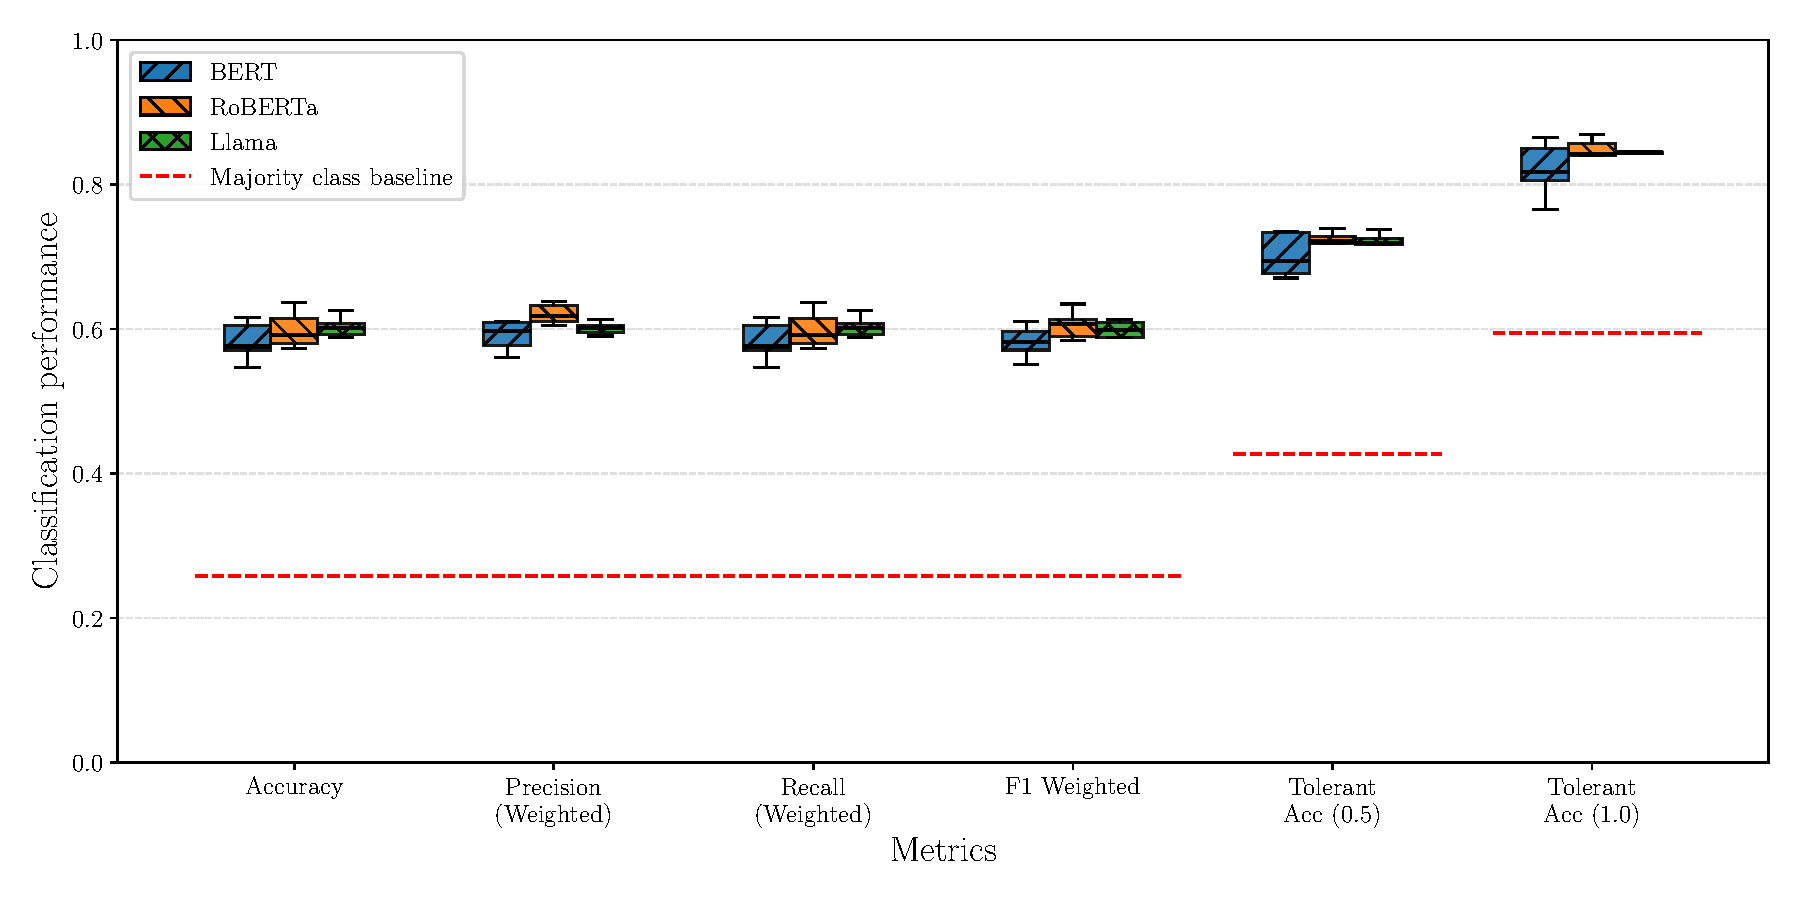
\includegraphics[width=1\linewidth]{img/results_boxplot_baselines.pdf}
    \caption{Article-level metrics across the five folds. Both baselines are drawn across every metric: red for Majority Class, violet for Uniform Random. Where the two coincide, as on Macro Recall at 0.20, the dashes alternate.}
\label{fig:results}
\end{figure}

Figure~\ref{fig:results} illustrates the results against the Majority Class Baseline (MCB, red) and the Uniform Random Baseline (RB, violet).
All models reach a standard accuracy around 0.60, more than double the MCB, with Mistral highest at 0.61. On macro-averaged performance Llama leads with $\mathrm{F1}_{\mathrm{macro}}$ of 0.55, followed by Mistral and RoBERTa at 0.54 and BERT at 0.52, all well above the RB of 0.19; the variance across folds is minimal (standard deviation about 0.02). Under the stricter tolerance ($\alpha = 0.5$), Mistral, Llama and RoBERTa reach approximately 0.72 against an adjusted MCB of 0.43.
With $\alpha = 1.0$ Llama reaches 0.84 and the others 0.82--0.83; the baseline is naturally higher here (0.60), so the gain is $+0.24$. Misclassifications are therefore rarely severe, typically involving adjacent labels.

\subsection{Biases in Article-level Reliability Prediction}
\label{subsec:error_analysis}

We examine whether classifiers consistently perform better in certain reliability classes than in others.

\begin{figure}[h!]
    \centering
    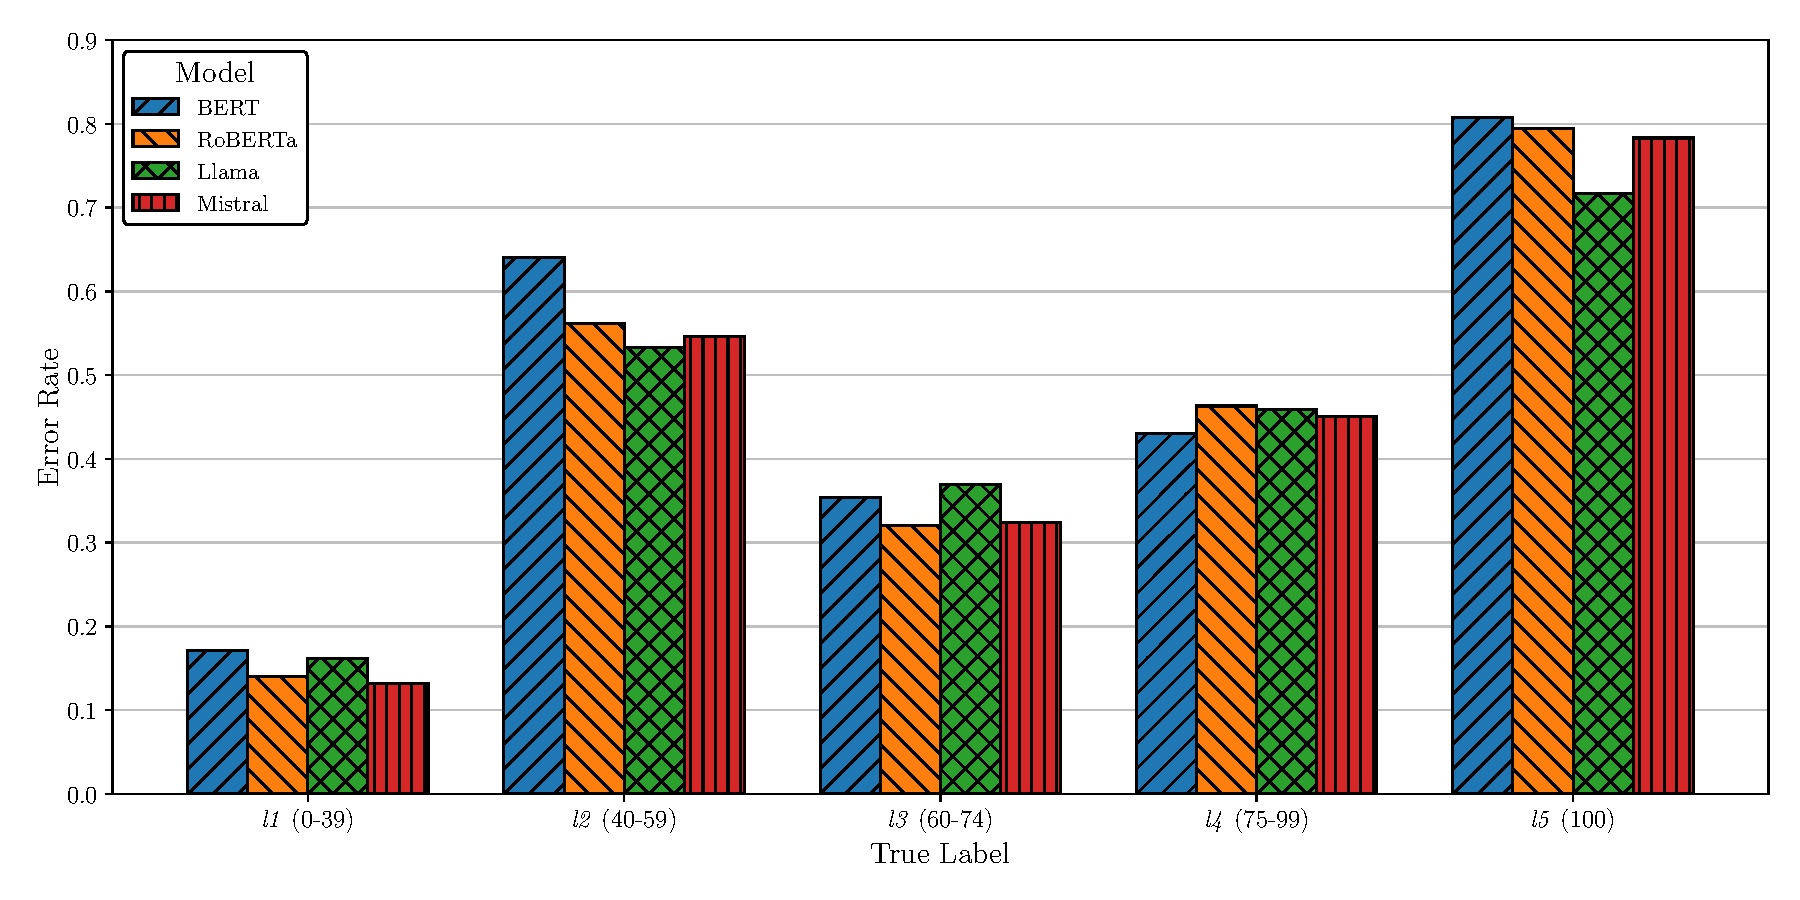
\includegraphics[width=1\linewidth]{img/error_rate_analysis.pdf}
    \caption{Per-class error rate, $(1-\mathrm{Recall}_l)$.}
    \label{fig:error_rate}
\end{figure}

Figure~\ref{fig:error_rate} highlights an asymmetry in prediction correctness. The lowest error rates are on $l_1$ ($< 0.20$), suggesting that highly unreliable content has recognizable structural features.
The highest-reliability articles ($l_5$) are the most challenging to recognize for the model, with error rates exceeding 70\%\footnote{Class $l_5$ only includes articles with a reliability score of 100, and is easily confused with $l_4$, which contains similarly high scores.}. Class $l_2$ also proves difficult, with an error rate of over 50\%, while $l_3$ sits in the middle at approximately 35\%.

These patterns remain consistent across all four models, suggesting that the biases are structural properties of the task rather than of a specific architecture; the Supplementary Material~\cite{suppmaterial2026} reports the error-direction analysis and the full confusion matrices.

\subsection{Influence of Political Leaning on Classification Errors}\label{subsec:politicalBias}
We examine whether classification errors are distributed evenly across the political spectrum. Political orientation is inherited from the publisher (Section~\ref{subsec:problemdef}), which allows a post-hoc analysis of how source-level alignment relates to article-level errors.

\begin{table}[t]
\centering
\begin{tabular}{lcr@{\hspace{2em}}l@{\hspace{2em}}c}
\toprule
\textbf{Model} & \textbf{Accuracy} & $\boldsymbol{\chi^2}$ & \textbf{$p$-value} & \textbf{Cramér's V} \\
\midrule
BERT & 58.27\% & 1684.13 & $<10^{-300}$ & 0.294 \\
RoBERTa & 60.34\% & 1418.31 & $<10^{-300}$ & 0.270 \\
Llama & 59.97\% & 1207.83 & $<10^{-250}$ & 0.249 \\
Mistral & 61.16\% & 1343.98 & $<10^{-280}$ & 0.263 \\
\bottomrule
\end{tabular}
\caption{Political leaning vs.\ classification correctness: $\chi^2$ test of independence with $p$-values, and Cramér's V as effect size.}
\label{tab:chi_square_results}
\end{table}

Error rates are computed separately within each political-leaning group, so they are not mechanically driven by differences in group size. They may nevertheless reflect differences in the distribution of reliability levels across groups.

All models exhibit systematic variation across political leanings: there are substantially higher error rates for far left and far right outlets (59--72\%) compared to lower rates for slightly right and non-labelled outlets (30--34\%), and intermediate error rates for slightly left articles (47--58\%).

A chi-square test of independence rejects, for every model, the hypothesis that correctness is independent of political leaning (Table~\ref{tab:chi_square_results}), with Cramér's~$V$ indicating a non-negligible association of broadly similar magnitude across models. Articles of the same outlet are not independent observations: they share both the leaning and the reliability label. We therefore repeat the test with one observation per publisher, namely whether its aggregated prediction is correct, and the association holds, with no expected count below five: $\chi^2$ ranges from 18.8 to 44.8, $p<10^{-3}$, and $V$ from 0.21 to 0.32. Leaning and reliability are themselves unevenly distributed in the corpus, and the overlap between them is incomplete: 142 of the 207 slightly right publishers sit in $l_1$, and no far-right publisher reaches $l_5$. A logistic regression that controls for the true reliability level, with standard errors clustered on the publisher, still leaves the two extremes with 4.0 to 6.5 times the odds of error of the non-labelled group, although the sparse cells limit how far the two variables can be separated; the Supplementary Material~\cite{suppmaterial2026} reports the coefficients, their intervals and the cell counts. A model trained on these labels may therefore reproduce the political structure of the corpus, regardless of whether the disparity originates in the annotations, in the article distributions, or in the model itself.

The Supplementary Material~\cite{suppmaterial2026} plots the Mean Error Direction for each orientation (Section~\ref{subsec:bias_methodology}), where positive values indicate overestimation of reliability and negative values underestimation.

Clear directional patterns emerge across all four models. Far Left and Far Right articles exhibit consistent overestimation, with mean signed errors ranging from +0.33 to +1.00, approaching a full reliability level. Slightly Left articles show systematic underestimation, with average values between -0.54 and $-0.82$. Slightly Right and non-labelled outlets display smaller, less consistent deviations; the Supplementary Material~\cite{suppmaterial2026} reports the corpus composition by leaning, the per-leaning error rates and the full confusion matrices stratified by political leaning.

\subsection{Stage 2: News Source Reliability Inference}
\label{subsec:stage2}

Publisher-level inference is the primary objective; the article-level predictors are
intermediate. We instantiate \(Agg\) as the mode of a publisher's predictions,
i.e.\ majority voting, which assigns the most frequent class as \(\hat{r}_P(p)\), on the
hypothesis that combining them offsets the noise of individual classifications.
Predictions are pooled across the five test folds, so each publisher's reliability
is inferred only from articles the model never saw in training.

\begin{figure}[t]
  \centering
  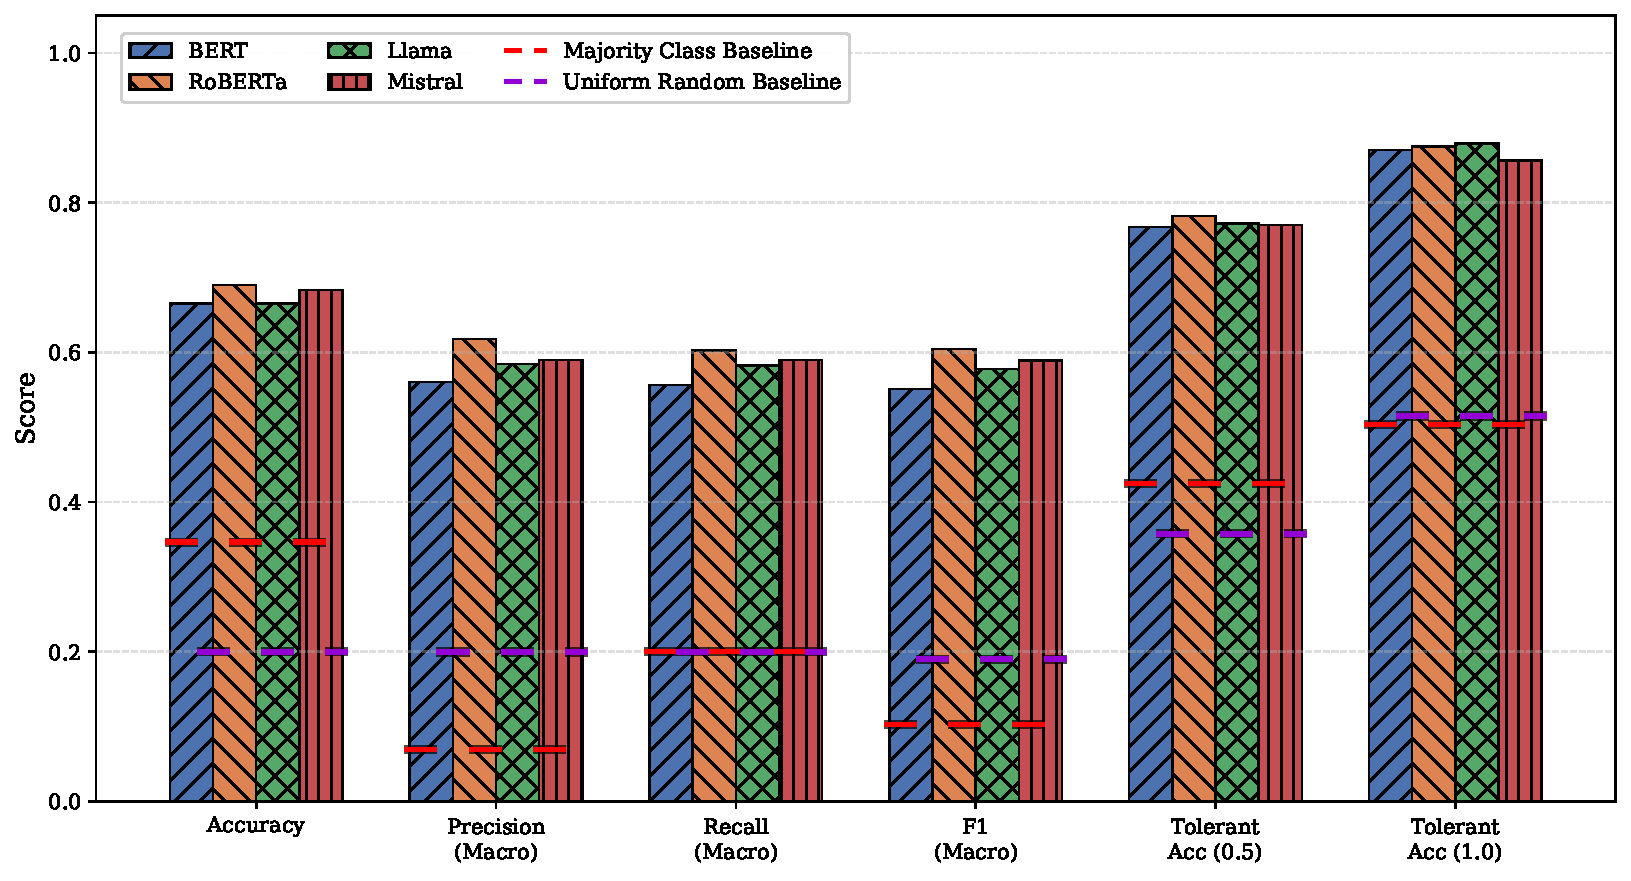
\includegraphics[width=\linewidth]{img/domain_metrics_comparison.pdf}
  \caption{Publisher-level metrics, with baselines drawn as in Fig.~\ref{fig:results}.}
  \label{fig:metrics}
\end{figure}

Figure~\ref{fig:metrics} presents the results against the same two baselines. The
majority-class reference differs across the three accuracy variants, since a constant
predictor also collects partial and then full credit under tolerance. Under full
tolerance the random baseline (0.52) in fact overtakes it (0.50), since a constant
predictor earns credit only next to its own level.

With an Accuracy of 0.69 RoBERTa leads, followed closely by Mistral at 0.68, more than triple the Random Baseline. On the same publishers, scoring one randomly chosen article per outlet already yields 0.63 to 0.66, so the vote itself adds 1.6 to 4.3 points; the rest of the gap from article-level accuracy reflects the change of evaluation unit. Considering $\mathrm{Accuracy}_{\mathrm{tolerant}}$ (1.0), Llama achieves the top score of 0.88, followed by RoBERTa (0.87) and Mistral (0.86), substantially outperforming the majority class baseline.

Most publisher-level errors involve adjacent levels, the most frequent being $l_5$ (High Credibility) predicted as $l_4$ (Generally Credible); the Supplementary Material~\cite{suppmaterial2026} reports full publisher-level confusion matrices and a detailed error analysis.




\section{Theory of Change}
\label{sec:theoryofchange}

Work on misinformation is not socially beneficial by default. We therefore state
what we expect this work to change, what must hold for it to do so, and how it
may cause harm.
\paragraph{The Need and What We Claim About It}
Expert ratings rely largely on manual assessment, leaving publishers outside their
coverage unrated. This gap motivates automation, but expanding coverage is not
itself the contribution of this paper. Instead, we change how the task is
formulated and evaluated. Reliability labels apply at the publisher level, yet much
computational work predicts them one article at a time and does not always keep
outlets apart between training and test, so reported performance may not
generalize to unseen sources. We therefore formulate the task at the publisher
level, enforce publisher-disjoint splits, and aggregate evidence across multiple
articles. Under
this stricter setting, our best method achieves 0.69 accuracy on unseen publishers
(Section~\ref{subsec:stage2}); most errors involve adjacent reliability levels, and
larger models show no consistent advantage in our experiments. The protocol and the
accompanying audit are released as reusable code, so that the change we propose can
be applied to corpora and label scales other than ours.


\paragraph{Preconditions and Their Plausibility}
The applicability of our approach depends on four conditions, whose plausibility
varies across settings. \textbf{The reference labels must be appropriate for the
intended use}: our models reproduce the NewsGuard scale and therefore inherit its
editorial judgements. Our experiments assess whether these labels can be predicted,
not whether the scale itself is a definitive measure of reliability. \textbf{Predictions
must be interpreted at the publisher level}: since article labels are inherited from
their sources, neither the supervision nor the article-level accuracy supports
claims about individual articles. \textbf{Sufficient textual evidence must be
available}: the approach needs multiple articles per publisher, which may limit it
for small, recent or infrequently publishing outlets. \textbf{Generalization must be
validated in the target domain}: our evidence concerns English-language political
news, and other languages, domains or periods require further evaluation.


\paragraph{Negative Externalities}
Our experiments reveal one potential source of harm: error rates vary systematically
across political-leaning groups (Section~\ref{subsec:politicalBias}), reaching
59--72\% for far-left and far-right outlets, compared with 30--34\% for slightly
right and non-labelled outlets. Among misclassified instances, the models also tend
to overestimate reliability at both political extremes and underestimate it for
slightly left-leaning outlets. These disparities should not be attributed to
political leaning alone, because leaning and reliability are unevenly distributed in
the corpus and cannot be fully separated by our analysis. Nevertheless, deploying the
models without accounting for this uncertainty could reproduce or amplify the
observed disparities.

Two additional risks concern how the predictions are presented and used. First,
assigning a single level on a five-point scale may convey more precision than the
models support, particularly because they struggle to distinguish \(l_4\) from
\(l_5\) (Section~\ref{subsec:error_analysis}). Second, once an automated score
influences rankings or access to resources, publishers may adapt their writing to
superficial cues learned by the model without improving the underlying editorial
practices.


\paragraph{Scope of the Evidence}
Our evaluation shows how accurately the approach predicts reliability labels for previously unseen publishers under a publisher-disjoint protocol. It does not establish whether those predictions improve human assessment in practice, how publishers should be prioritized for expert review, or when the system should abstain for lack of textual evidence; answering these would require a deployment-oriented evaluation with explicit decision rules and human assessors. We therefore present the approach as a potential source of decision support, not as a validated replacement for expert evaluation. The reporting these conditions imply is released as a checklist alongside the code, so that they can be applied rather than only read.

\section{Discussion and Conclusion}
\label{sec:conclusions}
Under a strict publisher-disjoint protocol, our findings show that language models capture generalizable signals of publisher reliability from articles alone. The substantially larger Mistral 24B does not consistently outperform smaller architectures, and its 1,024-token context window, four times the limit used for the others, brings no measurable gain. Since Mistral also differs in size and epochs, this does not isolate the effect of context length, but neither larger models nor longer inputs overcome the limits imposed by weak supervision. Publisher reliability is therefore better modelled as a collective signal that stabilises when evidence is aggregated across a source than as a property of isolated articles.

Future research should extend this framework to multilingual settings, explore confidence-aware aggregation strategies, and develop training objectives tailored to ordinal classification. The value of such systems, however, will not be settled by accuracy alone. Whoever builds one has to show where its errors fall across the political spectrum, which is why we report that disparity alongside the scores.

\begin{credits}
\ifanonymous
\else
  \subsubsection{\ackname}
  This work is partially supported by the IIT-CNR internal project SIMULARE
  `SIMULAzione delle Reazioni alla disinformazionE con LLM'.
\fi

\subsubsection{Data and Code Availability}
The supplementary document, the evaluation code, the fold assignment, the
aggregate statistics and a deployment checklist are at
\url{https://anonymous.4open.science/r/supplementary-material-DD54/}. The
NewsGuard labels are licensed to us and cannot be redistributed. Article texts are the publishers' copyright, so we release only their URLs. We do not
publish predicted reliability for named outlets either: at the error rates
reported here such a list would be the harm this paper argues against.

\subsubsection{\discintname}
The authors have no competing interests to declare.
\end{credits}

\bibliographystyle{splncs04}
\bibliography{bibliography}

\end{document}
